\documentclass[
	12pt,				% tamanho da fonte
	oneside,			% para impressão em recto e verso. Oposto a oneside
	a4paper,			% tamanho do papel. 
	english,			% idioma adicional para hifenização
	brazil,				% o último idioma é o principal do documento
	]{abntex2}

% ---
% Pacotes fundamentais 
% ---
\usepackage{lmodern}			% Usa a fonte Latin Modern
\usepackage[T1]{fontenc}		% Selecao de codigos de fonte.
\usepackage[utf8]{inputenc}		% Codificacao do documento (conversão automática dos acentos)
\usepackage{indentfirst}		% Indenta o primeiro parágrafo de cada seção.
\usepackage{color}				% Controle das cores
\usepackage{graphicx}			% Inclusão de gráficos
\usepackage{microtype} 			% para melhorias de justificação
\usepackage{multicol}
\usepackage{multirow}
\usepackage[brazilian,hyperpageref]{backref}	 % Paginas com as citações na bibl
\usepackage[alf]{abntex2cite}	% Citações padrão ABNT
\usepackage{listings}
\usepackage{float}

\lstset{
  showspaces=false,
  showtabs=false,
  breaklines=true,
  showstringspaces=false,
  breakatwhitespace=true,
  commentstyle=\color{green},
  keywordstyle=\color{blue},
  stringstyle=\color{red},
  basicstyle=\ttfamily
}

% --- 
% CONFIGURAÇÕES DE PACOTES
% --- 

% ---
% Configurações do pacote backref
% Usado sem a opção hyperpageref de backref
\renewcommand{\backrefpagesname}{Citado na(s) página(s):~}
% Texto padrão antes do número das páginas
\renewcommand{\backref}{}
% Define os textos da citação
\renewcommand*{\backrefalt}[4]{
	\ifcase #1 %
		Nenhuma citação no texto.%
	\or
		Citado na página #2.%
	\else
		Citado #1 vezes nas páginas #2.%
	\fi}%
% ---

% ---
% Informações de dados para CAPA e FOLHA DE ROSTO
% ---
\titulo{Prática 10: Otimização com Array Pool}
\autor{Pedro Inácio Rodrigues Pontes}
\local{Belo Horizonte, Brasil}
\data{2025}
\instituicao{%
  Universidade Federal de Minas Gerais
  \par
  Colégio Técnico
  \par
  Curso Técnico em Desenvolvimento de Sistemas}

\definecolor{blue}{RGB}{41,5,195}

\makeatletter
\hypersetup{
     	%pagebackref=true,
		pdftitle={\@title}, 
		pdfauthor={\@author},
    	pdfsubject={\imprimirpreambulo},
		colorlinks=true,       		% false: boxed links; true: colored links
    	linkcolor=blue,          	% color of internal links
    	citecolor=blue,        		% color of links to bibliography
    	filecolor=magenta,      		% color of file links
		urlcolor=blue,
		bookmarksdepth=4
}
\makeatother

\renewcommand{\thesection}{\arabic{section}}
\setlength{\parindent}{1.3cm}
\setlength{\parskip}{0.2cm} 

\makeindex


\begin{document}

\selectlanguage{brazil}
\frenchspacing 

\imprimircapa

{
\ABNTEXchapterfont

\textual

% ----------------------------------------------------------
% Introdução (exemplo de capítulo sem numeração, mas presente no Sumário)
% ----------------------------------------------------------
\section{Introdução}

O objetivo do presente trabalho foi a otimização de um código que simulava o processamento de imagens e a aplicação de um filtro \textit{blur} nelas. O código possuía 2 classes - Program e ImageProcessor -, além de uma struct PixelRGB. O componente no qual foi objetivada alteração era a classe ImageProcessor.

\section{Desenvolvimento}

\subsection{Versão Não Otimizada}
Antes de ser otimizado, o código apresentava uma criação excessiva de arrays, que poderiam simplesmente ser reutilizados usando array pool.

\begin{lstlisting}
public static void ProcessImages()
{
    Console.WriteLine("Iniciando processamento de imagens (versão trivial)...");
    
    for (int imageIndex = 0; imageIndex < TOTAL_IMAGES; imageIndex++)
    {
        PixelRGB[,] originalImage = GenerateSyntheticImage(imageIndex);
        PixelRGB[,] blurredImage = ApplyBlurFilter(originalImage);
        SaveImage(blurredImage, $"processed_{imageIndex}.jpg");
    }
    [...]
}

private static PixelRGB[,] GenerateSyntheticImage(int seed)
{
    var image = new PixelRGB[IMAGE_HEIGHT, IMAGE_WIDTH];
    var random = new Random(seed);
    
    for (int y = 0; y < IMAGE_HEIGHT; y++)
    {
        for (int x = 0; x < IMAGE_WIDTH; x++)
        {
            image[y, x] = new PixelRGB(
                (byte)random.Next(256),
                (byte)random.Next(256),
                (byte)random.Next(256)
            );
        }
    }
    return image;
}

private static PixelRGB[,] ApplyBlurFilter(PixelRGB[,] original)
{
    int height = original.GetLength(0);
    int width = original.GetLength(1);
    var blurred = new PixelRGB[height, width];
    
    for (int y = 0; y < height - 1; y++)
    {
        for (int x = 0; x < width - 1; x++)
        {
            blurred[y, x] = PixelRGB.Average(
                original[y, x],
                original[y, x + 1],
                original[y + 1, x],
                original[y + 1, x + 1]
            );
        }
    }
    return blurred;
}
\end{lstlisting}

\subsection{Versão Otimizada}
Os arrays reutilizados via ArrayPool foram implementados para GenerateSyntheticImage e ApplyBlurFilter, os quais geravam uma quantidade enorme de arrays temporários, sobrecarregando o GC (garbage collector).

Após a correção e aplicação das devidas alterações (ArrayPool não suporta arrays bidimensionais), o código ficou desta forma:

\begin{lstlisting}
public static void ProcessImages()
{
    Console.WriteLine("Iniciando processamento de imagens (versão otimizada)...");

    var pool = ArrayPool<PixelRGB>.Shared;
    PixelRGB[] blurred = pool.Rent(TOTAL_PIXELS);
    PixelRGB[] imageArray = pool.Rent(TOTAL_PIXELS);

    try
    {
        for (int imageIndex = 0; imageIndex < TOTAL_IMAGES; imageIndex++)
        {
            GenerateSyntheticImage(imageIndex, imageArray);
            ApplyBlurFilter(imageArray, blurred);
            SaveImage(blurred, $"processed_{imageIndex}.jpg");
        }
    }
    finally
    {
        pool.Return(blurred);
        pool.Return(imageArray);
    }
    [...]
}

private static void GenerateSyntheticImage(int seed, PixelRGB[] image)
{
    var random = new Random(seed);
    for (int y = 0; y < IMAGE_HEIGHT - 1; y++)
    {
        int rowStart = y * IMAGE_WIDTH;
        for (int x = 0; x < IMAGE_WIDTH - 1; x++)
        {
            image[rowStart + x] = new PixelRGB(
                (byte)random.Next(256),
                (byte)random.Next(256),
                (byte)random.Next(256)
            );
        }
    }
}

private static void ApplyBlurFilter(PixelRGB[] original, PixelRGB[] blurred)
{
    for (int y = 0; y < IMAGE_HEIGHT - 1; y++)
    {
        int rowStart = y * IMAGE_WIDTH;
        int nextRowStart = (y + 1) * IMAGE_WIDTH;
        for (int x = 0; x < IMAGE_WIDTH - 1; x++)
        {
            blurred[y * IMAGE_WIDTH + x] = PixelRGB.Average(
                original[rowStart + x],
                original[rowStart + x + 1],
                original[nextRowStart + x],
                original[nextRowStart + x + 1]
            );
        }
    }
}
\end{lstlisting}

\section{Resultados}

\begin{figure}[H]
    \centering
    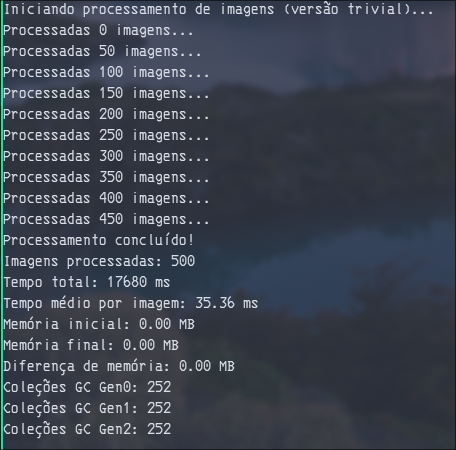
\includegraphics[width=1\textwidth]{imgs/versao-trivial.png}
    \label{Versão Não Otimizada}
\end{figure}

\begin{figure}[H]
    \centering
    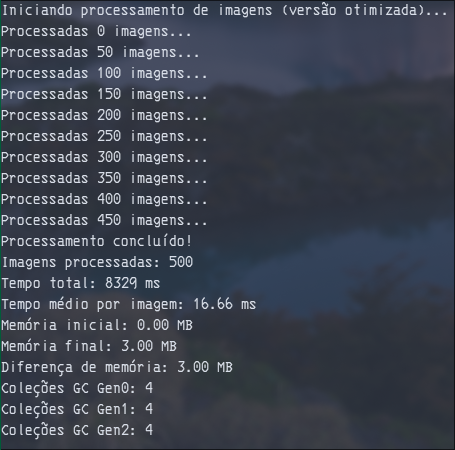
\includegraphics[width=1\textwidth]{imgs/versao-otimizada.png}
    \label{Versão Otimizada}
\end{figure}

\section{Conclusão}

A otimização foi alcançada. As alterações de memória inicial e final foram insignificantes nas duas situações. O mais relevante foram a diferença do total de coleções realizadas pelo garbage collector, que passaram de 252 para 4, e o tempo de execução, que caiu pela metade.

\end{document}
